\section{Introduction}
%
Glimmer\footnote{{\it Glimmer} was originally an acronym, reflecting
  the project's origin within GENIE. The meaning of the acronym is no
  longer important, however.} is a set of libraries, utilities and
example climate drivers used to simulate ice sheet evolution. At its
core, it implements the standard, shallow-ice representation of ice
sheet dynamics. This approach to ice sheet modelling is
well-established, as are the numerical methods used. What is
innovative about Glimmer is its design, which is motivated by the
desire to create an ice modelling system which is easy to interface to
a wide variety of forcing climates (whether models or data), without
the user having to have a detailed knowledge of its inner
workings. This is achieved by several means, including the provision
of a well-defined code interface to the model\footnote{The {\it API},
in computer-speak.}, as well as the adoption of a very modular
design. The model is coded almost entirely in standards-compliant
Fortran 95, and extensive use is made of the advances features of that language.
%
\section{Model versions and development strategy}
\label{intro-versions}
%
This document describes Glimmer version 1.0.6. The model code is
developed using the Concurrent Versions System (CVS), in a
publicly-accessible repository hosted at the UK National
eScience Centre (NeSC)\footnote{http://forge.nesc.ac.uk/projects/glimmer}. Glimmer
users are encouraged to participate in model 
development and documentation.

The model code held on the CVS repository is in a state of continuous
development. However, pre-packaged, numbered \emph{releases} of the model are
made at regular intervals; these can be downloaded from the NeSC
project website. A release collects together developments to the
model as a single snapshot, making it easier for users and
developers to keep track of changes. The 1.0.$x$ series of releases form the stable
development branch: changes in 1.0.$x$ are restricted to bug-fixes or minor
enhancements to existing features. In addition, a more experimental
development branch is maintained, where new features can be
implemented and tested, and whose versions are numbered 1.5.0 upwards.

Note that releases are always given even version numbers, such as 1.0.2, 1.0.4,
etc. The state of the CVS repository between releases is assigned a notional
odd version number, such as 1.0.3, 1.0.5, etc. This holds true for
supplementary package releases (e.g. of \texttt{glimmer-doc}).
%
\subsection{Overview}
%
Glimmer consists of several components:
%
\begin{itemize}
\item {\bf GLIDE:} {\bf G}eneral {\bf L}and {\bf I}ce {\bf D}ynamic
  {\bf E}lements: the core of the model.  This component is the actual
  ice sheet model. GLIDE is responsible for calculating ice
  velocities, internal ice temperature distribution, isostatic
  adjustment and meltwater production. GLIDE needs some representation
  of the climate to run, provided by a {\it driver} program. The user
  may write their own driver code, or may use one of the four supplied
  drivers (see section \ref{subsec:climdrive} below). 
\item {\bf SIMPLE:} Simple climate drivers that implement the
  experiments of the first phase of the EISMINT project, with
  idealized geometry. 
\item {\bf GLINT:} {\bf Gl}immer {\bf Int}erface. Originally developed
  for the GENIE\footnote{Grid-ENabled Integrated Earth-system model:
  \texttt{http://www.genie.ac.uk/}} Earth System Model, GLINT allows
  the core ice model to be coupled to a variety of global climate
  models, or indeed any source of time-varying climate data on a
  lat-long grid. An example driver is provided to illustrate the use
  of GLINT, which uses temperature and precipitation data to drive a
  positive degree day (PDD) mass-balance model. 
\item {\bf EIS:} {\bf E}dinburgh {\bf I}ce {\bf S}heet climate driver
  based on a parameterization of the equilibrium line altitude,
  sea-level surface temperatures and eustatic sea-level change. 
\item {\bf EISMINT3:} An implementation of a later part of the EISMINT
  project, concerning the modelling of the Greenland ice sheet. 
\item {\bf GLUM:} {\bf G}Limmer {\bf U}seful {\bf M}odules, various
  utility procedures used by the other components. 
\item Visualisation programs using GMT\footnote{Generic Mapping Tools:
\texttt{http://gmt.soest.hawaii.edu/}}.
\end{itemize}
%
\begin{figure}[htbp]
  \centering
  \includegraphics[width=0.6\textwidth]{\dir/figs/glimmer.eps}
  \caption{Relationship between the various Glimmer components.}
  \label{ug.fig.glimmer}
\end{figure}
The relationship between the Glimmer components is illustrated in Figure \ref{ug.fig.glimmer}.
%
\subsection{Climate Drivers}
\label{subsec:climdrive}
The core ice sheet model, GLIDE, is connected to the climate via the
surface mass balance and temperature fields and (optionally) a scalar
value for eustatic sea level. These drivers can be derived from simple
assumptions, e.g. uniform mass balance or EISMINT tests, or from
climate model output, e.g. GENIE or a regional climate model. These
components, and how they relate to each other, are outlined in Figure
\ref{ug.glide}. 
%
\begin{figure}[htbp]
 \begin{center}
   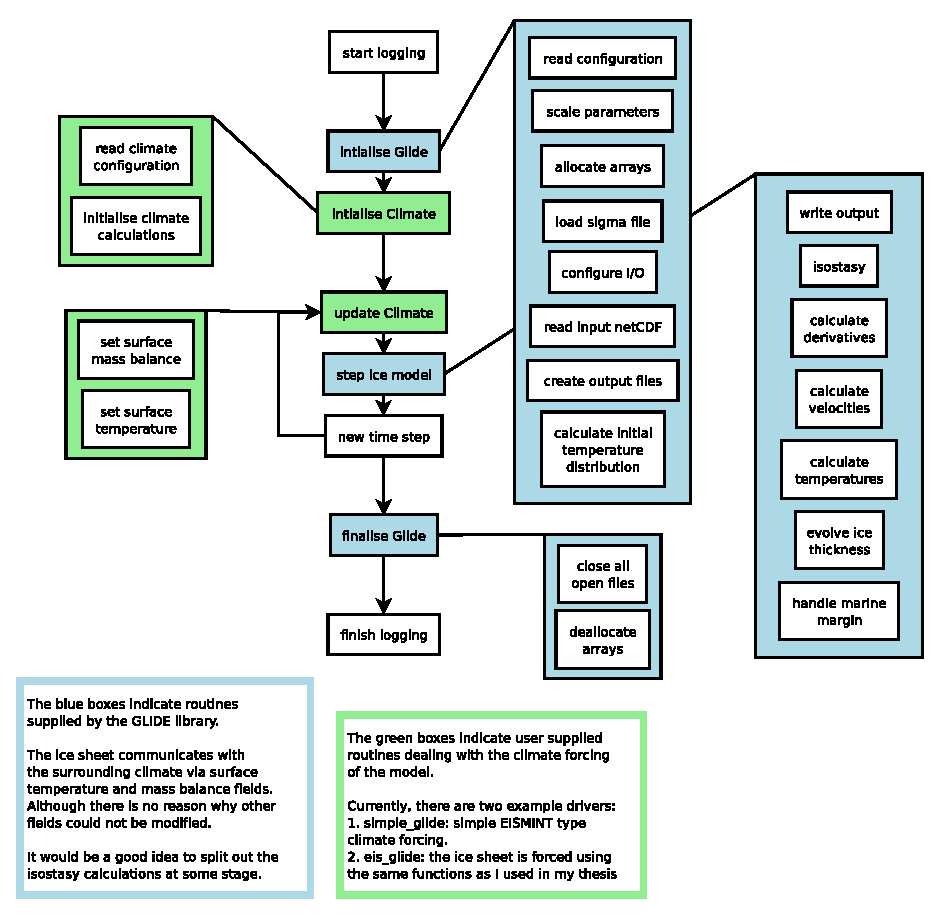
\includegraphics[width=0.9\textwidth]{\dir/figs/glide.eps}
 \end{center}
 \caption{Outline of the GLIDE and Climate components.}
\label{ug.glide}
\end{figure}
%
\subsection{Configuration, I/O and Visualisation}
In general terms, each component is configured using a configuration
file. The format of these files is consistent and easy to read.
At run-time, model configuration is printed to a log file.  

2D and 3D data is read/written to/from netCDF files using the CF
(Climate-Forecast) metadata
convention\footnote{\texttt{http://cf-pcmdi.llnl.gov/}}.
NetCDF is a scientific data format for storing multidimensional data
in a platform- and language-independent binary format. The CF
conventions specify the metadata used to describe the file contents. 

Many programs can process and visualise netCDF data, e.g. OpenDX,
Matlab, IDL, etc. Additionally, the Glimmer code bundle contains GMT
scripts written in Python to visualise the output.
